\section{Extension to non-planar fractures}
\label{section: Chapter4/nonplanar}

While in several practical cases, such as in layered formation, the assumption of planar fractures is recommended \cite{mcclure2020planar}, in many others, a general treatment that allows for non-planar growth in needed. However, in the context of the multi-resolution approach presented herein, this extension requires additional challenges to be addressed. In the last Section of this work, these challenges are discussed and a skeleton of a possible modified algorithm is described. A simplified nonplanar fracture problem in 2D is then used to test it. Although the result is favorable, the extension of this algorithm to full 3D problems requires additional modifications whose robustness is unclear. 

\subsection{Overview of a propagation algorithm for non-planar fractures}\label{basicNonplanarAlgo}

In Section \ref{section: Chapter4/algo}, the algorithm \ref{fig:MR_planar_algo} showed how to use the multi-resolution method to treat planar fractures in 3D. To extend it to non-planar cases, at a minimum, the following parts must be modified. 

\begin{itemize}
    \item First, the algorithm for tracking the damage in the front elements described in subsection \ref{frontTrackingAlgo} must be revisited, considering that the damage field is not planar. That definitely breaks the hypothesis of the damage volume criterion and also introduces pathological cases that make the applicability of the topological criterion more difficult.
    
    \item The update of the geometry becomes more complex for the same reason. Given a nonplanar damage field in an element, how to insert a planar\footnote{While it is possible to develop embedded methods that allow for curved cuts inside elements, those are rarely used in practice due to the complex integration techiniques needed. Because of that, in the current work, while strong assumptions on the embedded scheme are avoided, the focus is on first-order (i.e planar cuts) methods.} cut in the mesh that represents it well?
    
    \item Finally, while for planar cuts the continuity of the fracture surface is always guaranteed, in nonplanar case, local (element-wise) approximations of the damage field with discrete cuts may lead to gaps in the fracture surface, such as the ones shown in Figure \ref{fig:gaps}.
\end{itemize}

To address the first bullet point, one can start with the topological criterion proposed in \ref{frontTrackingAlgo}, where the number of edges and faces with damage above a threshold is used. In general, if the damage band is small compared to the global element size, there is likely no ambiguity in the identification of cutting points. However, if the regularization length or the mesh size in the local problem are not very small, some difficulties may arise. For example, a wide damage band approaching the element diagonally may cut two adjacent edges as shown in Figure \ref{fig:pathological_case}. This leads to a configuration where the number of cut edges and faces is large albeit the actual global element is not yet fractured. 

\begin{figure}
    \centering
    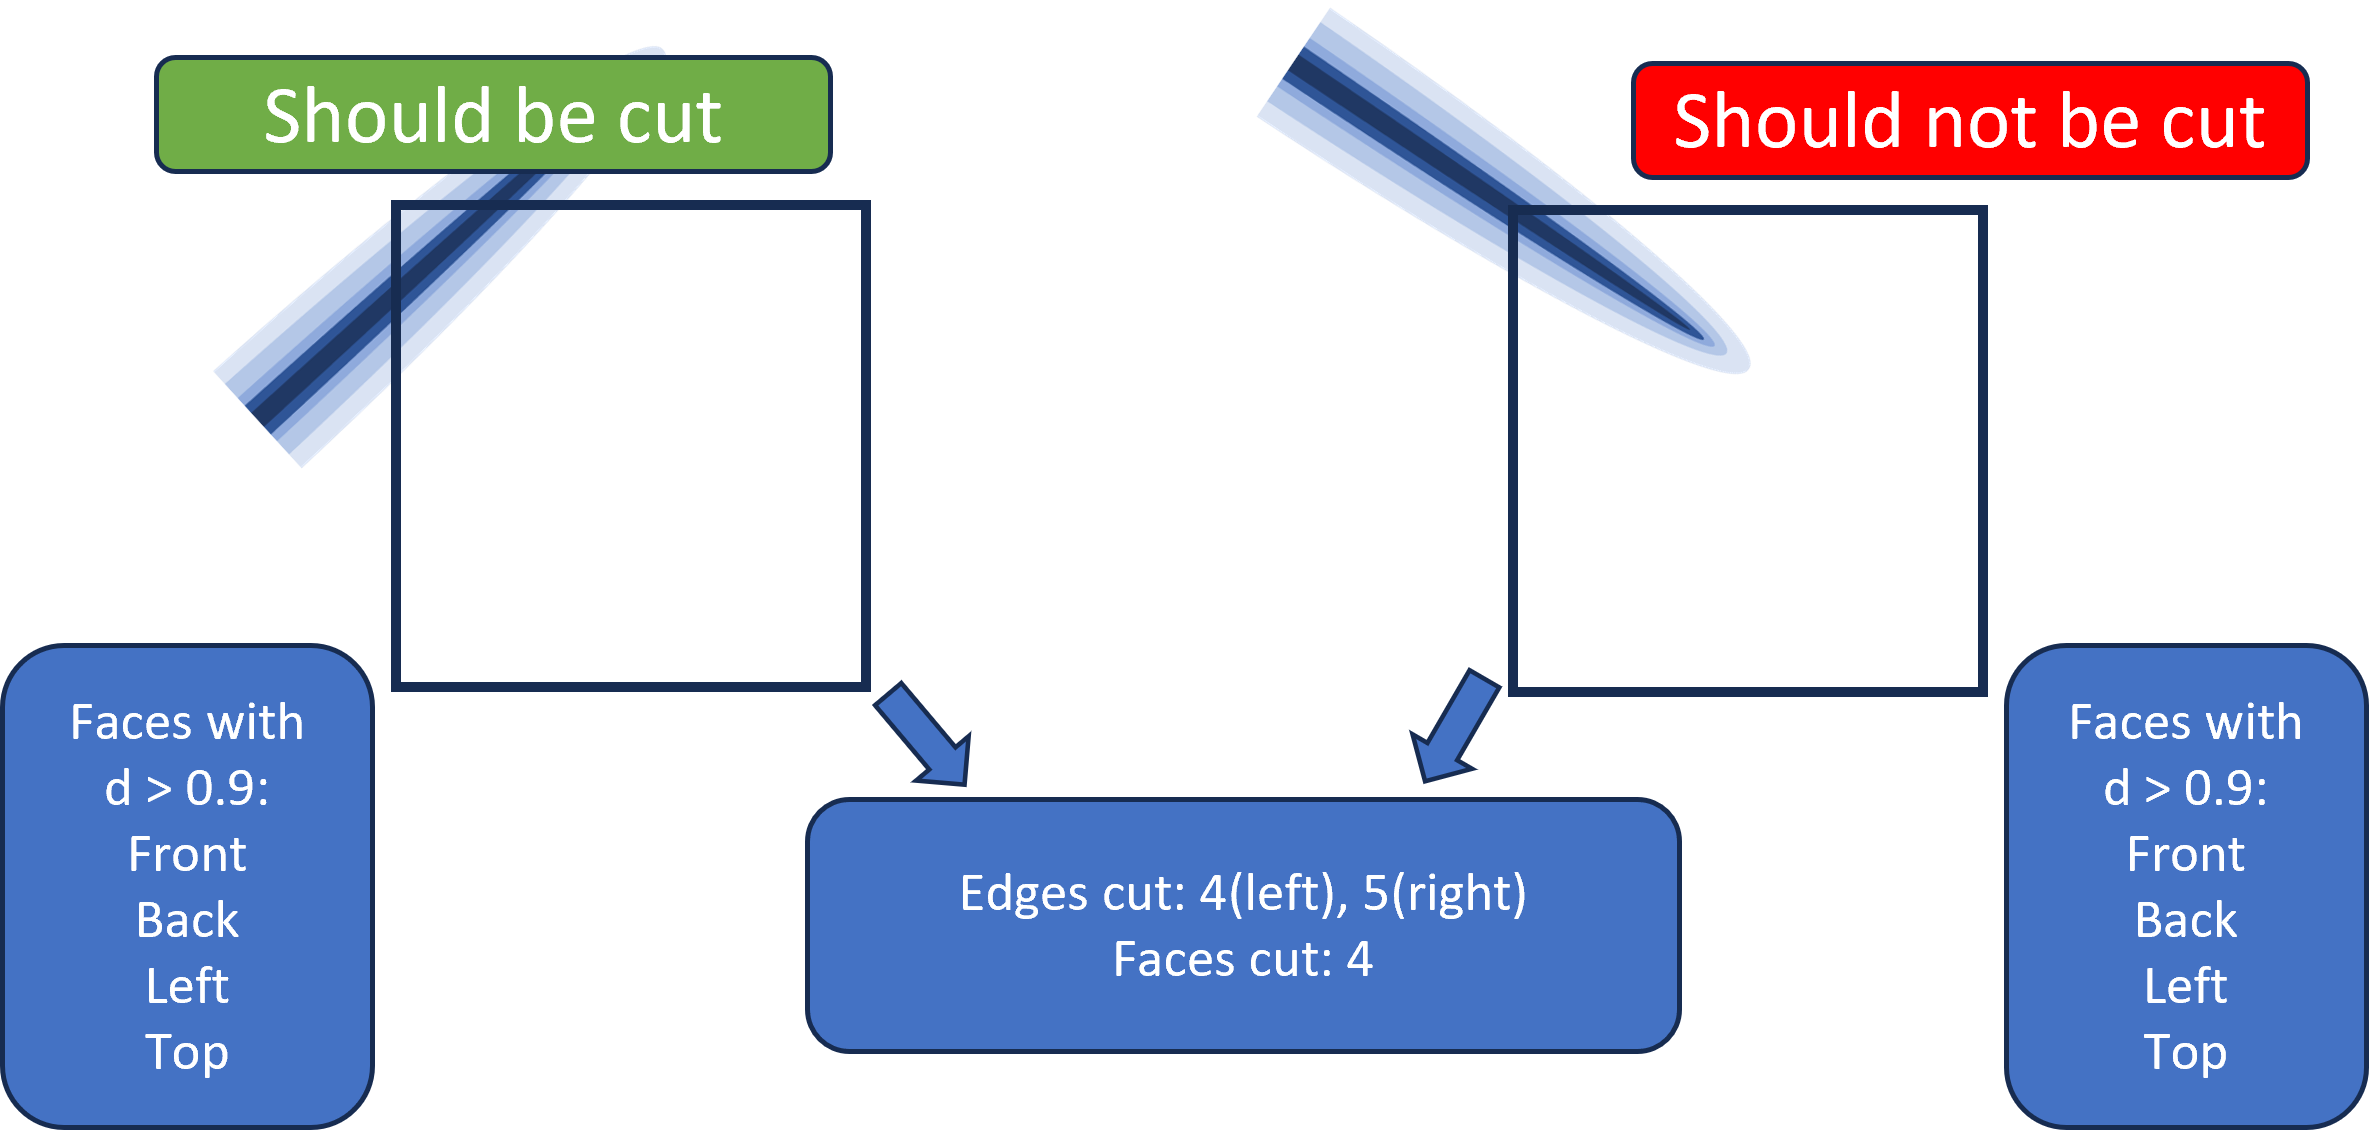
\includegraphics[width=\linewidth]{Chapter4/figures/nonplanar/pathology.png}
    \caption{This figure shows a pathological case for the topological criterion proposed in \ref{frontTrackingAlgo}. The element on the right is only partially damaged, however, the counts of cut edges and faces are higher than the ones for the element on the left, which is indeed fully cut.}
    \label{fig:pathological_case}
\end{figure}%

Overcoming this limitation likely requires the use of information about the damage in neighboring elements. One approach, used in the example problem shown next, keeps the topological criterion the same, but introduces a check on the cutting angle that is obtained after an element is cut. This check consists of comparing the normal to the new cut with the neighboring fractured elements. If the normals are too different (i.e $\textbf{n}\cdot\textbf{n}_{neighbor} << 1$), then, this newly inserted cut is assumed to be due to a pathological case and then removed. The respective element is only considered for cutting again when the number of damaged faces increases. This check will be refered to as ``the angle check".

This heuristic relies on the assumption that fractures do not kink strongly over element boundaries, which is only true if the fracture curves have a large radius of curvature compared to the global element size. 

Now, in terms of the second bullet point, regarding the extraction of the cutting plane from a damage field, an optimization algorithm such as \cite{geelen2018optimization} can be employed. In a nutshell, this method searchs over the space of planes embedded in an element and constructs an idealized damage profile around this plane, using the optimal profile\footnote{This is the profile for an AT-1 phase-field formulation.} given by $d(x) = (1-\text{dist}(x)/2\ell)^2$, where $\text{dist}(x)$ denotes the distance from $x$ to the plane. These idealized profiles are then compared to the actual damage field and the one which is closest in the $L_2$-sense is chosen to be the cutting plane for that damage field.

One must be careful when integrating this optimization approach with the angle check described above. That heuristic works under the assumption that an attempted cut on an element which is not yet fractured will lead to a cutting plane that does not conform well to its neighbors. If an optimization approach is employed, that might not always be true. For example, in the case shown in Figure \ref{fig:pathological_case}, the optimization approach can find the cutting plane induced by the partial fracture which will conform well to the existing cuts, even though the element is only partially cut.

So, in order to use the angle check, instead of applying the optimization method and then comparing the calculated plane with its neighbors, the idea of a coarser ``pre-cut'' is used. The idea of these pre-cuts is to rely only on the relative position of the cut identified in the element edges and faces by the topological criterion. This is done to ensure that, if one is dealing with a pathological case for the topological criterion, the pre-cut will indicate that and fail the angle check. In a 2D scenario, these pre-cuts can be obtained for example, by connecting the midpoints of the fractured faces. In 3D, the mapping becomes more complex. Figure \ref{fig:pre_cuts} shows the four basic ways that a plane can intersect a brick element, rotations and reflections also need to be included. The pre-cut to be chosen for an element in 3D can then be obtained by evaluating which of these best approximate the set of damaged faces computed by the topological criterion for that element (based on its damage field in the local scale). 

\begin{figure}[h]
    \centering
    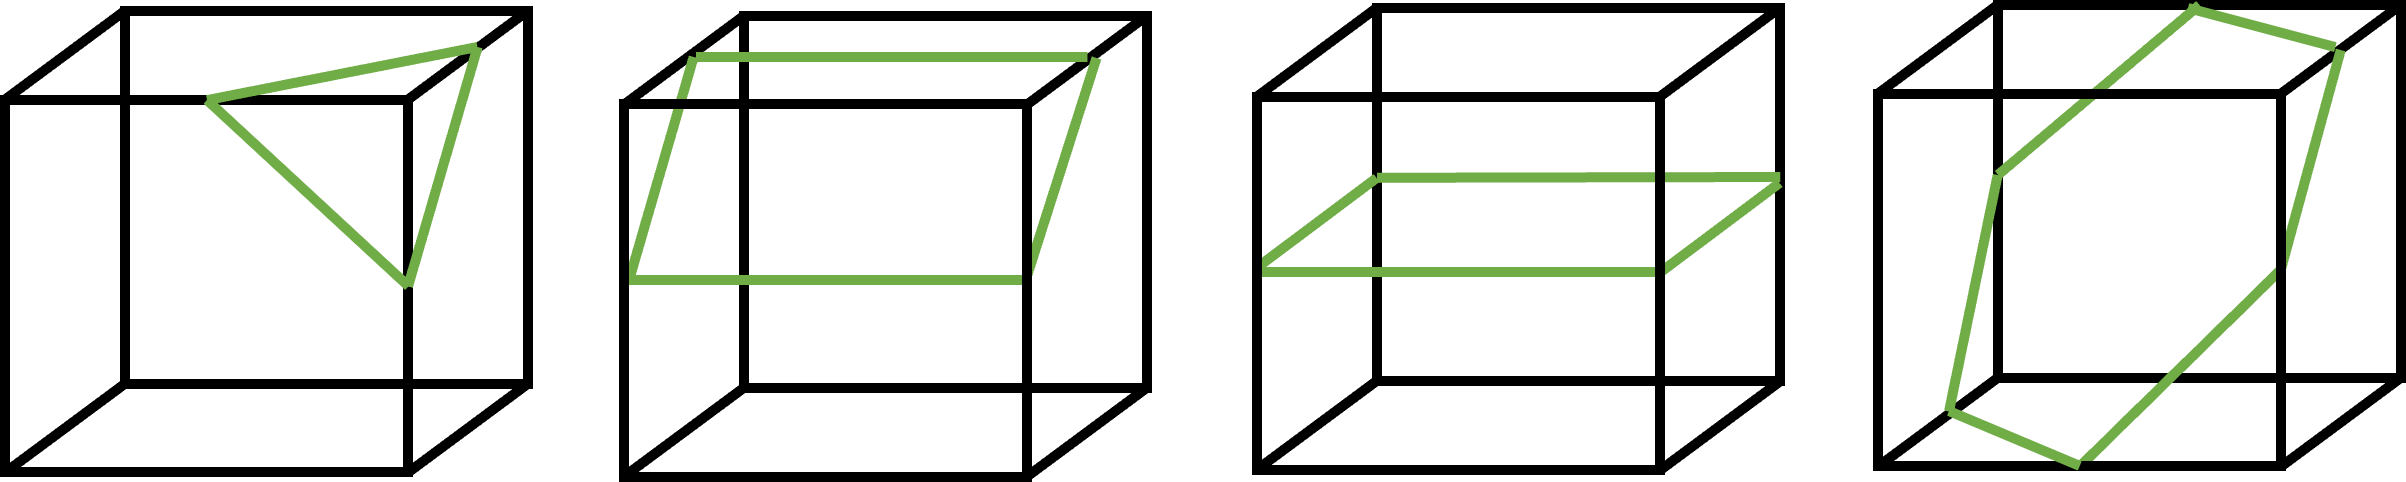
\includegraphics[width=0.8\linewidth]{Chapter4/figures/nonplanar/pre_cuts.png}
    \caption{Basic shapes for a planar cut in a brick element.}
    \label{fig:pre_cuts}
\end{figure}

Even with these modifications, the third and last bullet point, that concerns the continuity of the fracture surface must be addressed. For general embedded fracture approaches, continuity of the fracture surface is a necessary feature for the construction of the approximation space for the displacement field. This imposes serious complications to any type of algorithm that tries to construct surface increments on an element to element basis such as the one used here. However, the EFEM/EDFM approach used in this work and first proposed in \cite{cusini2021simulation} does offer a possible way to handle this issue. Unfortunately, that does break the generality of the multi-resolution approach with respect to the discretization techinique used in the global domain. 

By construction, the EFEM method does not assume continuity of the displacement field across element boundaries. In fact, the enrichment employed to represent the displacement jump does not interact with the neighboring elements and the final aperture might indeed be discontinuous. Still, the method does converge to the continuous solution in space. Figure \ref{fig:efem_apertures}, from \cite{cusini2021simulation} shows a typical aperture field computed with EFEM. This flexibility allows one to work with a fracture surface that has gaps in its geometry and still compute an accurate aperture field. 

\begin{figure}[h]
    \centering
    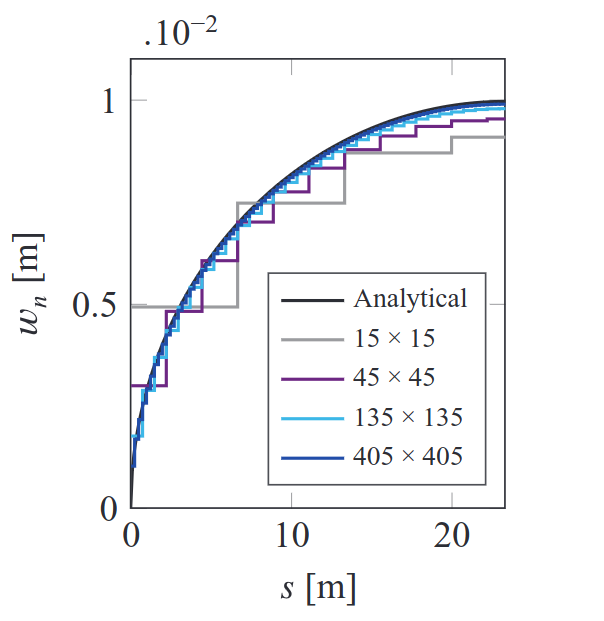
\includegraphics[width=0.5\linewidth]{Chapter4/figures/nonplanar/efem_aperture.png}
    \caption{This figure shows how the aperture field computed with EFEM approaches an analytical solution as the mesh is refined. Note that the aperture field is discontinuity across element boundaries. Courtesy from \cite{cusini2021simulation}}
    \label{fig:efem_apertures}
\end{figure}

On the other hand, for the computation of the flow problem, continuity is still required to calculate fluxes from a fracture cell to its neighbors. In fact, two compute the flux between two embedded cells, their common edge is used. That is, if one obtains a discontinuous fracture surface, there will be neighboring cells that do not share an edge and therefore, the flux between them will be zero.

Luckly, this issue can be circuvented by noting that the damage intersection on any edge is the same for all elements that contain that edge. Therefore, instead of computing the fluxes directly from the common edge of neighboring fracture cells, one can store the intersections of the damage field with the global element edges and use them to build segments in between two neighboring cells. These segments can them be used to compute the fluxes, ensuring that even neighboring cells that happen to be on a surface discontinuity still get a unique, meaningful flux. Figure \ref{fig:flux_calculations} shows two neighboring fracture elements that form a gap. In this case, the damage intersections D1 and D2 should be use to define the common edge that enters the flux calculation.

\begin{figure}[h]
    \centering
    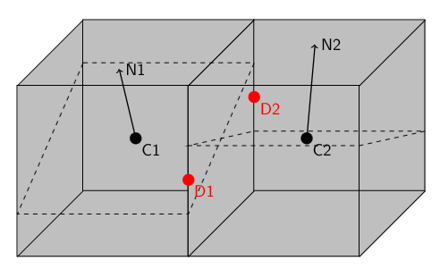
\includegraphics[width=0.6\linewidth]{Chapter4/figures/nonplanar/nonplanar_flux.png}
    \caption{Flux in discontinuous fracture surfaces. D1 and D2 are the intersections of the damage field with the edges and serve to define a line segment that can be used to calculate the flux between the two fracture elements.}
    \label{fig:flux_calculations}
\end{figure}

Combining all the workaround described in this Section, we can obtain an algorithm that extends algorithm \ref{fig:MR_planar_algo} to allow for the treatment of non-planar fractures with a multi-resolution scheme. These modification are displayed as an algorithm in Figure \ref{fig:nonplanar_algo}.

While this algorithm theoretically answers most of the challenges discussed in this Section, a full implementation for general 3D problems is not yet completed. Currently, only the first modification to the algorithm, which concerns the topological criterion and its enhancement with the angle check and pre-cuts is implemented and tested. The optimization scheme and the flux computations based on the damage interesections in the edges are left for future investigations. 

\begin{figure}[h]
    \centering
    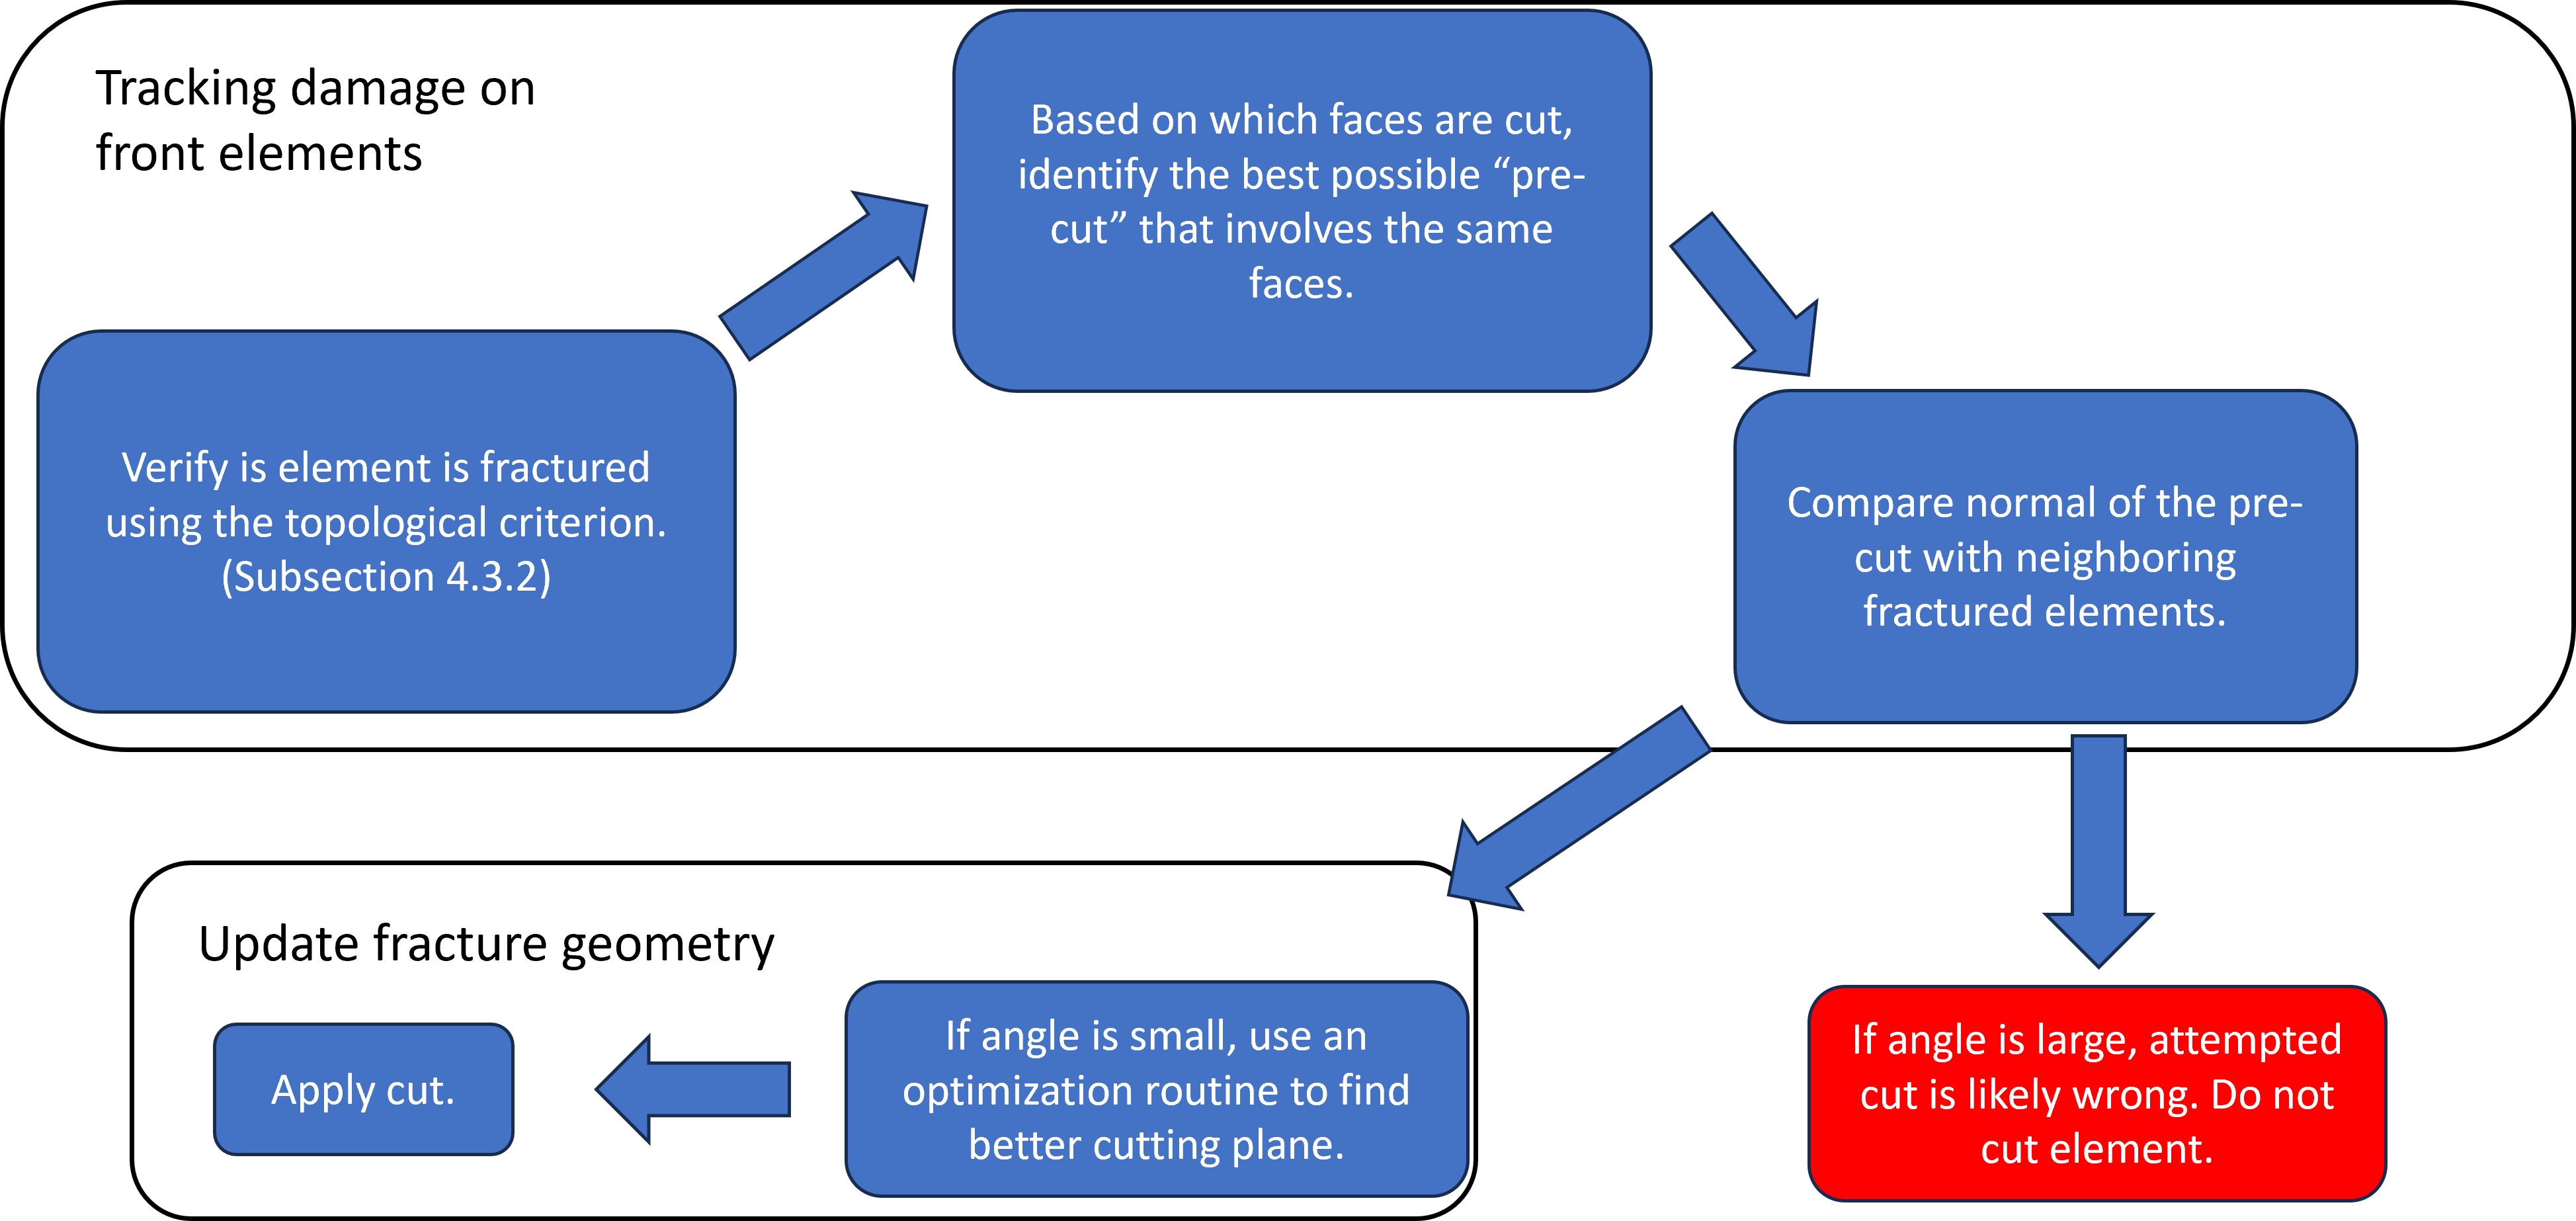
\includegraphics[width=\linewidth]{Chapter4/figures/nonplanar/nonplanar_algo.png}
    \caption{Enhancements to \ref{fig:MR_planar_algo} to allow for non-planar fracture propagation.}
    \label{fig:nonplanar_algo}
\end{figure}


In the next section, this simplification of the algorithm described above is applied to a 2.5D problem where the crack path is curved. It serves to check the efficacy of the proposed changes in the process of identifying the crack path. The fluid flow and poroelastic effects are turned off for simplicity.

\subsection{Example problem}

This subsection presents a small 2D problem used to test some features of the algorithm presented in \ref{basicNonplanarAlgo}. The problem consists of an edge crack in a square plate, which is pulled in the top edge by an inclined displacement $\Delta u$, at an angle of 45deg, as shown in Figure \ref{fig:nonplanar_schematic}. The bottom surface is held fixed while the sides are left with a zero traction boundary condition. The material properties and geometric parameters are given in Table \ref{material properties nonplanar}. All the fluid effects are removed, as the focus is only on the algorithm to track the fracture and insert the discrete cuts. The subdomain is set to be the entire domain, which simplifies the transfer of boundary conditions from the global to local problem. 

\begin{table}[h]
    \centering
    \caption{Material properties for non-planar fracture problem.}
    \begin{tabular}[t]{lcc}
    \hline
    &Value &Unit \\
    \hline
    Young's modulus ($E$)&16.0&GPa\\
    Poisson's ratio ($\nu$)&0.18&--\\
    Critical energy release rate ($G_c$)&2.5&$\text{N/m}$\\
    Regularization length ($\ell$)&0.04&$\text{m}$\\
    Applied displacement ($\Delta u$)&$2.0\times 10^{-5}$&$\text{m}$\\
    Initial crack length (a)&2.5&$\text{m}$\\
    Plate size (L)&5.0&$\text{m}$\\
    \hline
    \end{tabular}
    \label{material properties nonplanar}
\end{table}%

In terms of discretization, the coarser global mesh uniformly splits the domain in 21x21 elements, with the finer grid being 11 times smaller. That leads to a subdomain element whose size is 2 times smaller than the phase-field regularization length. The load increment used was $2.0\times 10^{-7}$ m. 

A very similar problem was studied in \cite{giovanardi2017hybrid}. Despite the differences in material properties, it serves as a reference solution for the crack path, which is the main quantity of interest for this analysis. So, their results are shown in Figure \ref{fig:reference result}. Despite the simplification in defining the cut direction, the discrete fracture is still capable of tracking the damage band quite well, as shown in Figure \ref{fig:crack_path}, displaying a great agreement with the reference solution. Interestingly, this problem involves multiple cases of the damage band approaching the diagonal of an element, which constitutes a pathological case, described previously. This shows that the correction based on the neighboring cutting angles is indeed useful and necessary in this type of approach.

A relative straightforward improvement can be done with the introduction of an optimization method, as discusssed in \ref{basicNonplanarAlgo} to produce cuts that better align with the damage band locally. However, the use of "crude" approximations (pre-cuts) is still important to test the angle criteria and prevent lighly damaged elements from being wrongly cut due to a pathological case, such as the one shown in Figure \ref{fig:pathological_case}.

One the downside, this example doesn't explore a lot of the difficulties that arise in general three-dimensional problems. 
First, creating a map between the damaged faces and the pre-cuts shown in Figure \ref{fig:pre_cuts} becomes much more difficult in 3D. In addition to that, the angle criteria may work well in cracks that evolve progressively as the one in this example, however, it may get into a ``locking" situation if two cracks are merging at an angle. This is, different neighbors may impose constraints in the cutting angle of an element that may be impossible to satisfy simultaneously. 

Overcoming these challegens likely requires a more severe reformulation of the algorithm used for planar fractures. One promising approach is to employ a global method of surface reconstruction after the solution of the phase-field problem. This is a research topic on its own, with important contributions developed in recent years, such as \cite{yang2021explicit, zeng2022tracking, xu2023reconstruct}. In the context of hybrid phase-field methods, the authors of \cite{eldahshan2021cipfar} used a global surface reconstruction to improve the simulation of ductile fracture. They used the gradient of the damage to guide the identification of a discrete fracture surface embedded in a triangular mesh. While the robustness of their reconstruction in the presence of crack merging and branching is still unclear, it certainly points to a promising direction that can be explored in the context of the multi-resolution approach for hydraulic fracture.

\begin{figure}[ht]
    \centering
    \begin{tikzpicture}
        \node {\pgfimage[interpolate=false,width=.4\textwidth]{/home/andre/projects/Dissertation/dissertation/Chapter4/figures/nonplanar/nonplanar_schematic.png}};
        \draw (-0.1\textwidth,0.04\textwidth) node {\large$a$};
        \draw (0.22\textwidth,0.0\textwidth) node {\large$L$};
        \draw (0.02\textwidth,0.23\textwidth) node {\large$\Delta\textbf{u}$};
    \end{tikzpicture}
    \caption{Schematic of the edge crack problem. The load of the top surface is inclined 45deg, which leads to a curved fracture path.}
    \label{fig:nonplanar_schematic}
\end{figure}

\begin{figure}[h]
    % \centering
    \begin{subfigure}{.45\textwidth}
      \centering
      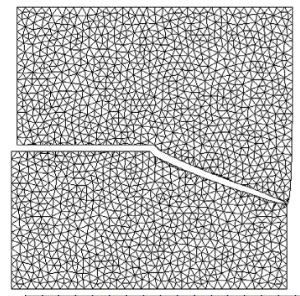
\includegraphics[width=0.765\linewidth]{Chapter4/figures/nonplanar/curved_crack_result_bianca.png}
      \caption{Crack path - Giovanardi et al. \cite{giovanardi2017hybrid}.}
      \label{fig:reference result}
    \end{subfigure}%
    \begin{subfigure}{.54\textwidth}
      \centering
      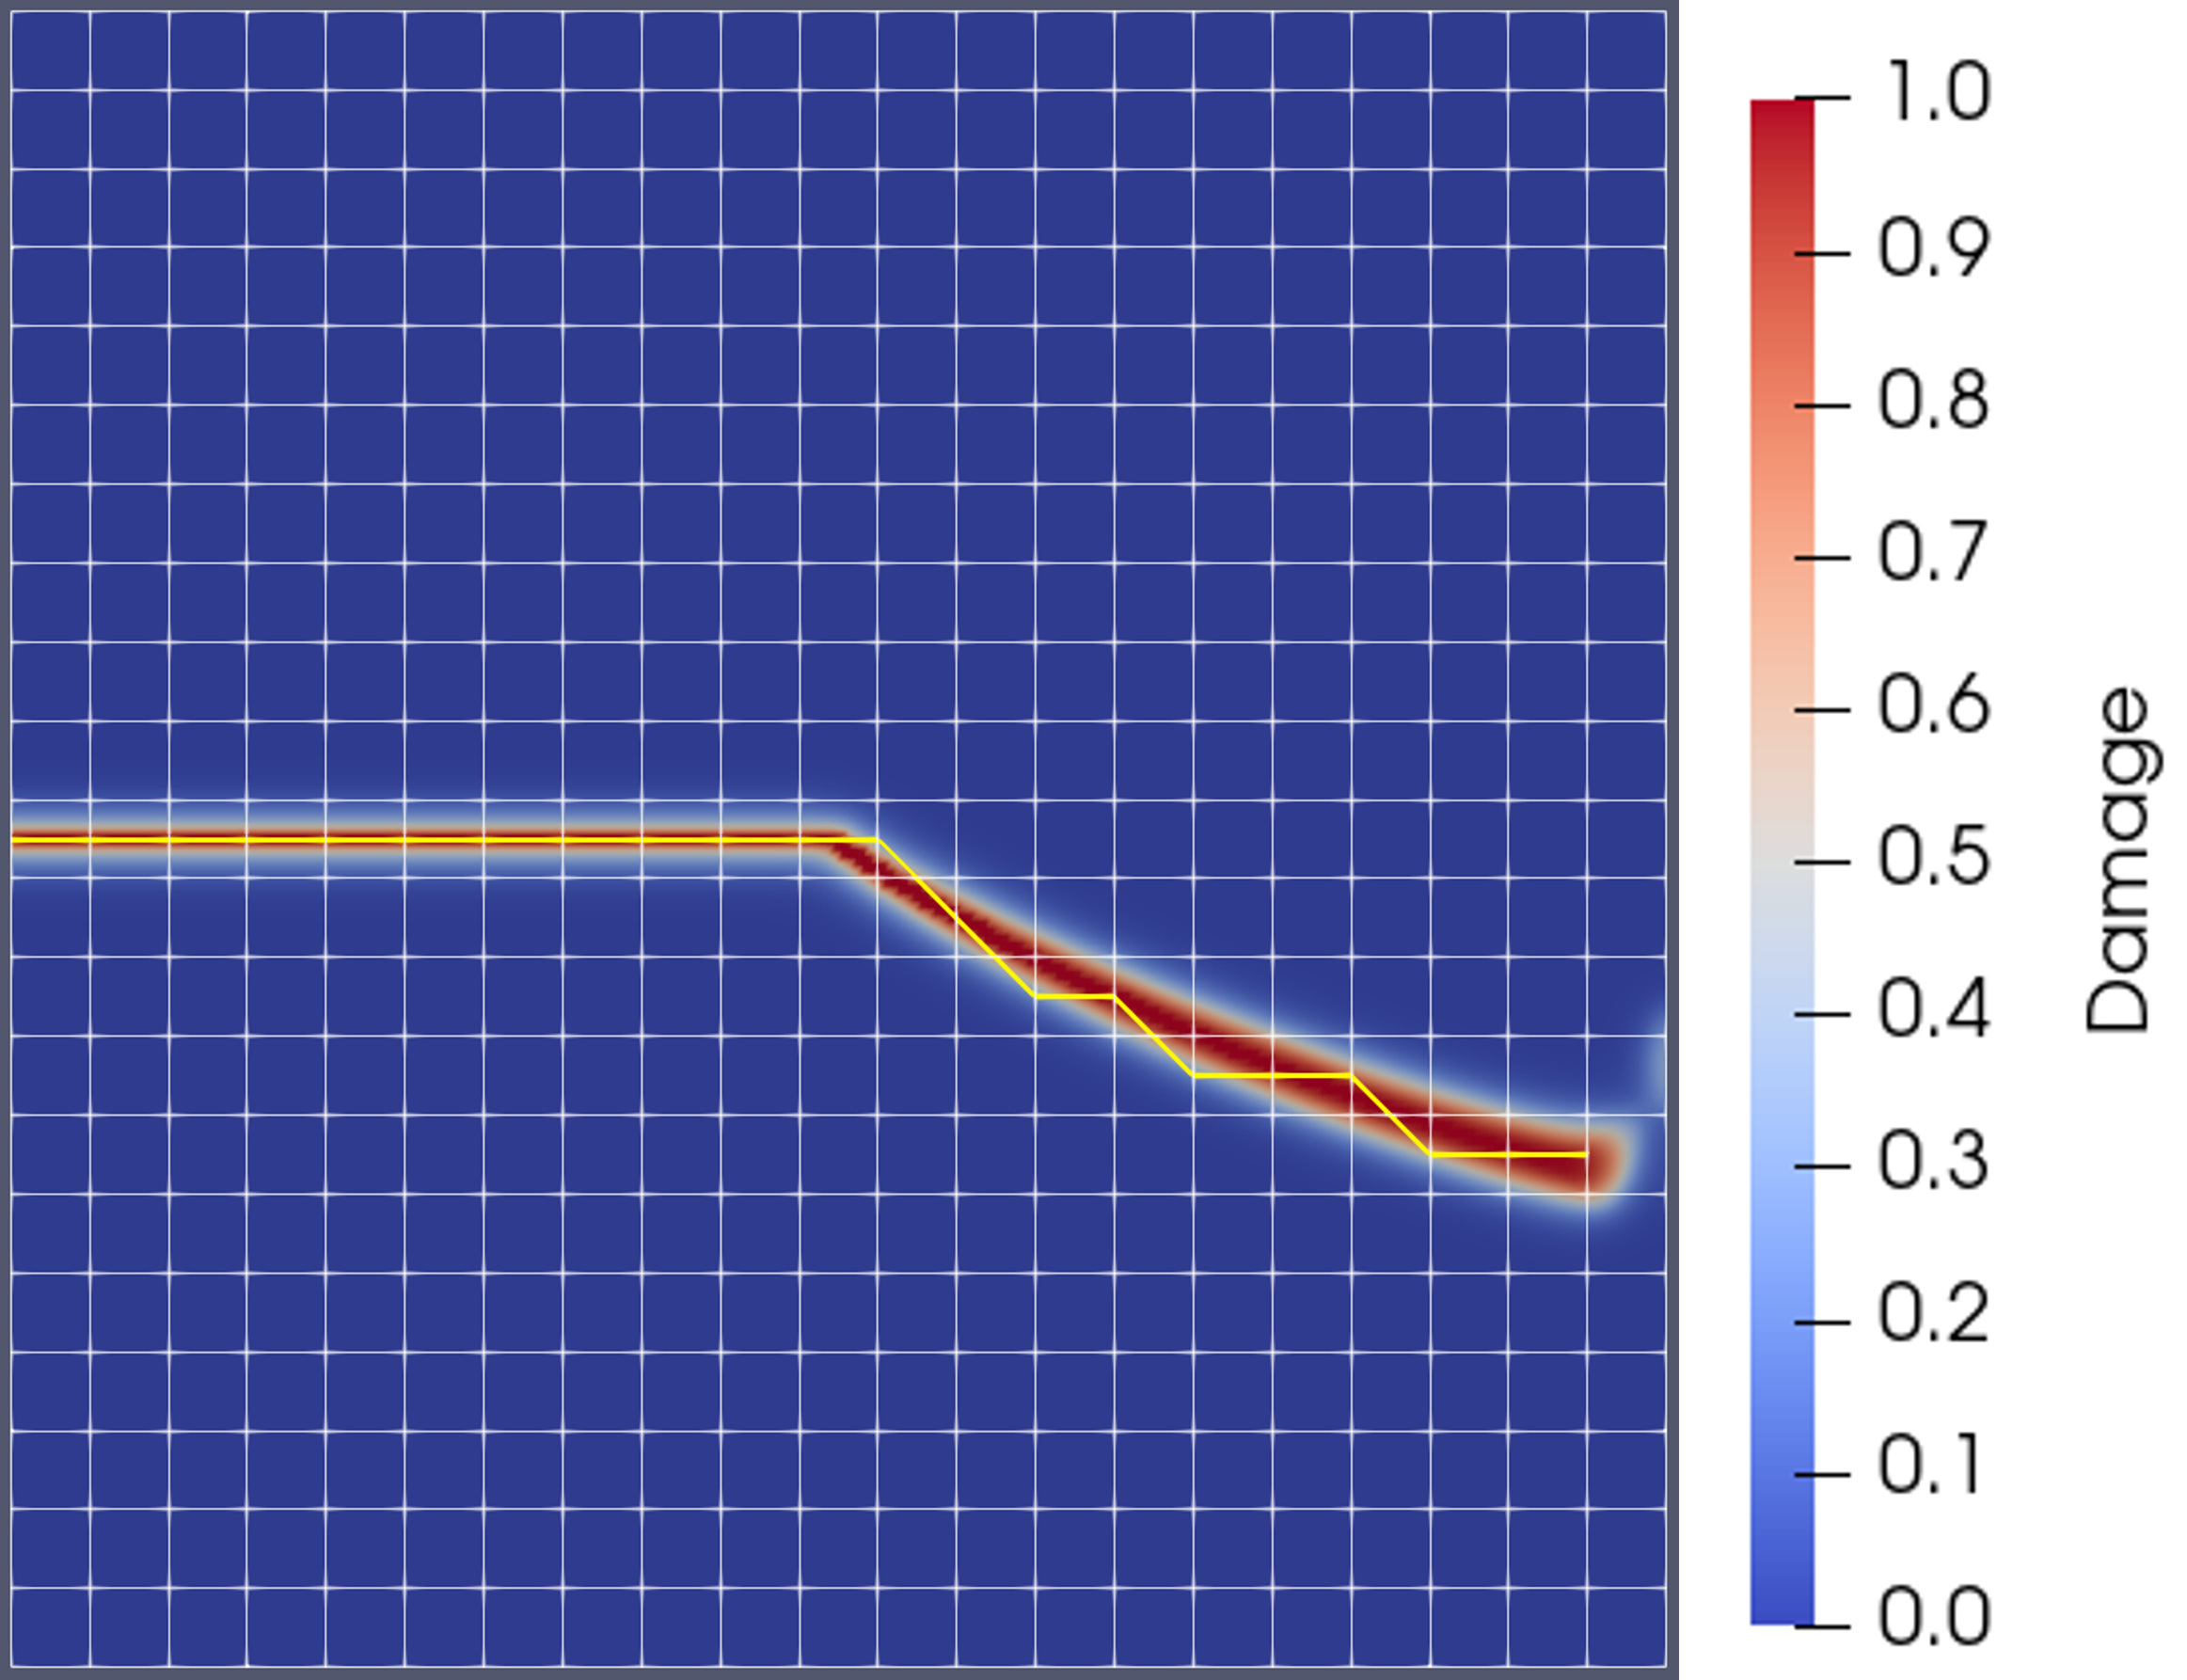
\includegraphics[width=0.83\linewidth]{Chapter4/figures/nonplanar/nonplanar_example.png}
      \caption{Crack path - current work}
      \label{fig:crack_path}
    \end{subfigure}%
      \caption{Comparision of the crack paths obtained for the edge crack problem. Despite the roughness of the crack path in (b), the overall path compares very well to the reference result.} 
      \label{fig:nonplanar_example}
\end{figure}